\documentclass[letterpaper,11pt]{article}
\oddsidemargin -1.0cm \textwidth 17.5cm

\usepackage[utf8]{inputenc}
\usepackage[activeacute,spanish, es-lcroman]{babel}
\decimalpoint
\usepackage{amsfonts,setspace}
\usepackage{amsmath}
\usepackage{amssymb, amsmath, amsthm}
\usepackage{comment}
\usepackage{float}
\usepackage{amssymb}
\usepackage{dsfont}
\usepackage{anysize}
\usepackage{multicol}
\usepackage{enumerate}
\usepackage{graphicx}
\usepackage[left=1.5cm,top=2cm,right=1.5cm, bottom=1.7cm]{geometry}
\setlength\headheight{1.5em} 
\usepackage{fancyhdr}
\usepackage{multicol}
\usepackage{hyperref}
\usepackage{wrapfig}
\usepackage{subcaption}
\usepackage{siunitx}
\usepackage{cancel}
\usepackage{mdwlist}
\usepackage{svg}
\pagestyle{fancy}
\fancyhf{}
\renewcommand{\labelenumi}{\normalsize\bfseries P\arabic{enumi}.}
\renewcommand{\labelenumii}{\normalsize\bfseries (\alph{enumii})}
\renewcommand{\labelenumiii}{\normalsize\bfseries \roman{enumiii})}


\begin{document}

\fancyhead[L]{\itshape{Facultad de Ciencias F\'isicas y Matem\'aticas}}
\fancyhead[R]{\itshape{Universidad de Chile}}

\begin{minipage}{11.5cm}
    \begin{flushleft}
        \hspace*{-0.6cm}\textbf{FI1000-1 Introducción a la Física Clásica}\\
        \hspace*{-0.6cm}\textbf{Profesor:} Ignacio Bordeu\\
        \hspace*{-0.6cm}\textbf{Auxiliares:} Javier Cubillos \& Berenice Muruaga\\
        \hspace*{-0.6cm}\textbf{Auxiliares taller:} Pablo González \& Alejandro Cartes\\
        \hspace*{-0.6cm}\textbf{Ayudante:} Amaru Moya\\
    \end{flushleft}
\end{minipage}

\begin{picture}(2,3)
    \put(366, 10){
\includegraphics[scale=0.9]{2020-1/Imágenes/logo/dfi-fcfm.pdf}}
\end{picture}

\begin{center}
	\LARGE\textbf{Taller \#5}\\
	\Large{Dinámica}
\end{center}

\vspace{-1cm}
\begin{enumerate}\setlength{\itemsep}{0.4cm}

\rfoot[]{pág. \thepage}

\item[]

\item
\begin{multicols}{2} 
    Una partícula de masa $m$ que se puede mover sin roce sobre una superficie horizontal está unida por una cuerda ideal de largo $L$ a un resorte ideal de constante elástica $k$ y largo natural $\ell_0$ nulo, el cual está unido por el otro extremo a un bloque de masa $M$. Este bloque está apoyado sobre una superficie que está ubicada a una distancia $H$ abajo del plano que contiene a la primera partícula. Calcule la máxima velocidad angular $\omega$ con que la partícula debe girar en un movimiento circular uniforme para que el bloque no se despegue del suelo.
    
    \columnbreak
    \begin{figure}[H]
        \centering
        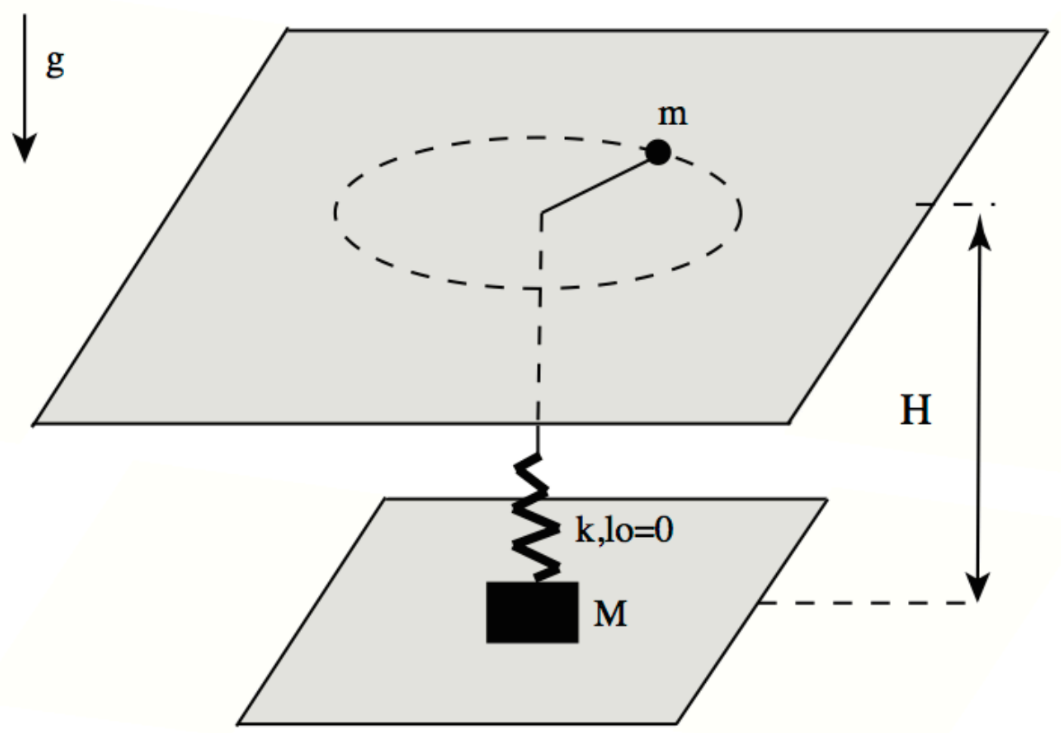
\includegraphics[width=0.8\linewidth]{2022-2/Imagenes/Taller5/resorte.png}
    \end{figure}
\end{multicols}

\item Una esfera de masa $m$ es mantenida en la posición $A$ por dos cuerdas. Sea $T_A$ la tensión de la cuerda indicada. Se corta la cuerda horizontal y el péndulo oscila hasta la posición $B$. ¿Cuál es la razón de las tensiones $T_B/T_A$?

\begin{figure}[H]
    \centering
    \svgpath{../../2021-2/img/aux4}
    \includesvg[width=0.4\linewidth]{pendulos.svg}
\end{figure}


% Para imágenes vectoriales -> el texto tiene que estar en LaTeX
% \begin{figure}[htbp]
%   \centering
%   \svgpath{../Imagenes/ejercicios}  -> .. irse pa'trás 
%   \includesvg{ej5.svg}
% \end{figure}

\end{enumerate}
\end{document}
